\section{Contexto}
\subsection{Construcción de interfaces de usuario usando el patrón MVC}

	\subsubsection{MVC}
	El patrón Modelo-Vista-Controlador (MVC) es un estilo de arquitectura de
	software que separa el modelo de dominio, la UI,
	y la relación entre ellos \emph{(Controlador)} en tres componentes distintos
	\cite{burbeck87}.
	
	La idea principal de MVC, y que influyó a la mayoría de los frameworks de
	presentación posteriores, es la de Presentación Separada \emph{(Separated
	Presentation)}, que consiste en hacer una división clara entre objetos de 
	dominio que modelan nuestra percepción del mundo real y objetos de presentación, 
	que son los elementos UI que vemos en la pantalla. 
	Esto nos brinda una clara separación de responsabilidades entre interfaz,
	lógica de negocio y control. Además nos permite soportar múltiples
	presentaciones para un mismo modelo de información \cite{reenskaug79}.
	\bigskip
	
	En la figura \ref{mvc} se describen los tres componentes.  
	
	\begin{figure}[h]
		\centering
		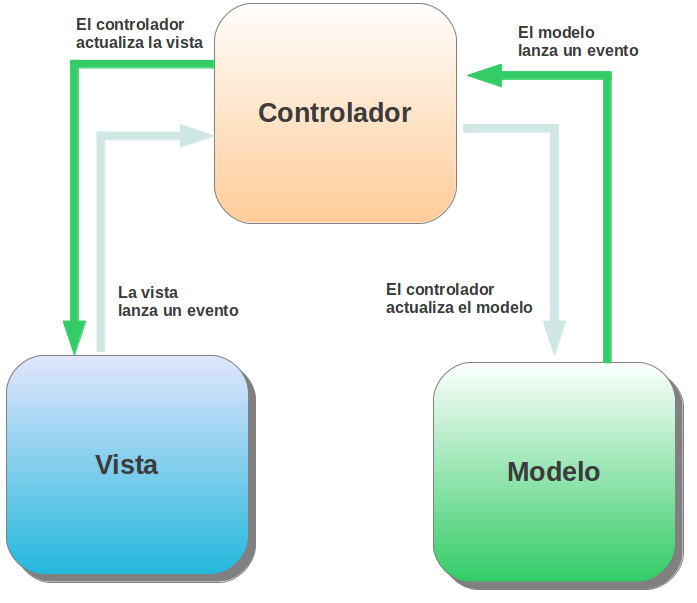
\includegraphics[width=300px, height=300px]{img/mvc} 
		\caption{Esquema MVC}
		\label{mvc}
	\end{figure}  
	
	\begin {itemize}
	
		\item {\bf Modelo}
			El modelo maneja el comportamiento y la información del dominio de la
			aplicación, responde a los pedidos de información sobre su estado, 
			y responde a las instrucciones para cambiar su estado. 
			
			
		\item {\bf Vista}
			La Vista muestra la información del modelo al usuario e interactúa y recibe
			las acciones del mismo.
			
		\item {\bf Controlador}
			Es el intermediario entre el modelo y la vista.
			Captura los eventos emanados tanto del modelo como de la interfaz, y coordina
			la interacción entre ambos.
			
	
	\end {itemize}

\subsubsection{Eventos}
\label{Eventos}

	Un evento es un suceso en el sistema, tal como una interacción del usuario con
	la máquina, o un mensaje enviado por un objeto.  
	El sistema maneja el evento enviando el mensaje adecuado al objeto pertinente. 
	
	\begin{quote}
	
	\begin{description}
	   
	\item [Objetivo] Definir una dependencia 1:n de forma que cuando el objeto
		1 cambie su estado, los n objetos sean notificados y se actualicen
		automáticamente, a estos objetos se los conoce como \emph{listener}. Esto me
		permite una comunicación entre objetos con muy bajo acoplamiento.
	
	\item [Motivación] En la construcción de interfaces de usuarios, se tiende
		a separar los objetos de presentación (vistas) de los objetos de dominio, de
		forma que se puedan tener varias vistas sincronizadas de la misma información.
	
	\end{description}
	\end{quote}
	
	Muchas implementaciones del patrón MVC se construyen utilizando el 
	patrón Observer. Donde el patrón Observer se contruye
	utilizando eventos \cite{Gamma1995}.

%\comment{Hay MVC's que en su implementación no utilizan eventos: TODO citar.}%


\subsubsection{Binding}
\label{binding}

	El \emph{binding} es una conección de propiedades entre dos objetos. 
	Nos permite sincronizar los valores de las propiedades de dos objetos
	diferentes, por ejemplo: vista y modelo. Habitualmente esto se logra a través
	del uso de eventos.
	Cada vez que el valor de una propiedad cambia, el objeto notifica, dispara un
	evento, y todas las propiedades que estén conectadas a él,
	reflejan los cambios automáticamente, dando la posibilidad de transformar y
	validar la información.\\
	También automatiza el procedimiento del traspaso de la información del
	modelo a la interfaz y viceversa.\\
	
	A continuación en la figura \ref{fig:binding} se describe el esquema de
		\emph{binding}
		
		\begin{figure}[h]
			\centering
			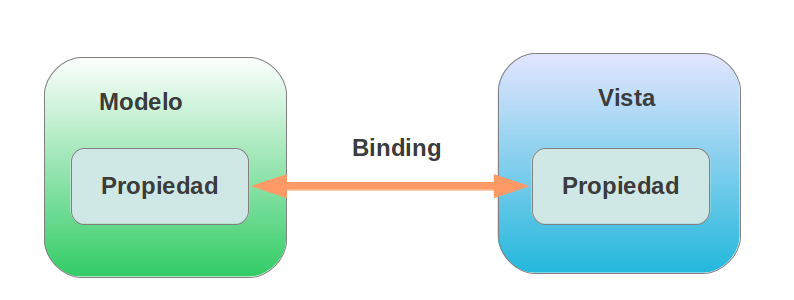
\includegraphics[width=300px]{img/binding}
			\caption{Esquema Binding}
			\label{fig:binding}
		\end{figure}
		
		\bigskip
	
	La ausencia de \emph{binding} implica mayor trabajo  y como consecuencia
	conlleva mayor tiempo de desarrollo en  traspasar la información de los
	objetos de dominio hacia los componentes de la interfaz gráfica y viceversa, repitiendo muchas lineas de código.
	
	Podemos tener información inconsistente, como por ejemplo, al mostrarse la interfaz,
	muestra el valor actual de la propiedad de un objeto de dominio, y después el
	objeto de dominio cambia el valor de su propiedad, la interfaz no se actualiza,
	y la información queda inconsistente.
	
	\bigskip
	
	Se pueden diferenciar dos tipos de \emph{binding}:
	
	\begin {itemize}
	
		\item {\bf Unidireccional}
		El \emph{binding} unidireccional permite que los cambios en la propiedad de
		origen (modelo) actualicen automáticamente la propiedad de destino (vista),
		pero los cambios en la propiedad del modelo no se propagan de nuevo a la
		propiedad de la vista.
		Este tipo de \emph{binding} es adecuado si el control que se va a enlazar es
		de sólo lectura de forma implícita.		
		
		\item {\bf Bidireccional}
		El \emph{binding} bidireccional permite que los cambios realizados en la
		propiedad del modelo o de la vista se actualicen automáticamente en el
		otro. Este tipo de \emph{binding} es adecuado para formularios modificables u
		otros escenarios de interfaz de usuario totalmente interactivos.
		Esto es posible, gracias a la utilización de los eventos, tanto desde el
		dominio como de la interfaz.
	
		En nuestro trabajo nos enfocamos en este tipo de binding.
		 
	
	\end {itemize}
	


\subsubsubsection{Limitaciones}
	Para poder utilizar el \emph{binding}, se necesita que los objetos de dominio, 
	conozcan el concepto de eventos.
	
	Otro problema que aparece frecuentemente es que el binding en su versión más 
	sencilla modifica los objetos directamente, por lo que al cancelar una operación 
	se debe volver al estado anterior, y este proceso es repetitivo y propenso a errores. 

	
\subsubsection{Framework Arena}
	Arena es un Framework sencillo que implementa los principios de diseño y
	organización de interfaces de usuario que se ven en la materia Creación de
	Interfaces de Usuario\footnote{Creación de Interfaces de Usuario
	es una materia del Núcleo avanzado obligatorio de la Tecnicatura
	Universitaria en Programación Informática de la Universidad Nacional de
	Quilmes}.
	
	Esta creado con fines educativos y por lo tanto se focaliza en la puesta en
	práctica de los conceptos mas relevantes.